\lhead{\emph{\leftmark}}  % Set the left side page header to "Abbreviations"
\chapter{Evaluation}
\label{chap:evaluation}
% how far can we umplify a new system
In order to ensure that the results presented in this thesis are of high engineering quality and are as valid as possible from a scientific perspective, several approaches need to be followed. We validated our reverse engineering approach  by studying the application of our approach on various software systems. We adopted a \textbf{four-phase validation process}with the following steps:

\begin{description}

\item[Testing Phase]
Unit testing is carried out following a Test Driven Development approach (TDD).

\item[Pre-validation Phase]
Small Java systems written in high quality Java code, with known corresponding models, are employed to validate the accuracy of the transformations performed by the Umplificator.

\item[Initial Phase]
Medium and large  open-source projects are employed to validate the accuracy of the transformations and mapping rules. This set of open source projects will be known as the \textbf{'training set'}. The goal of this phase is to ensure the correctness and precision of the transformations on the training set.

\item[Machine Learning-Based Phase]
In this phase, we umplify a set of randomly selected systems, the\textbf{'testing set'} and assess the extent to which our transformations still work. We document the errors encountered during this phase of validation.

\end{description}

In general all four of the above phases are conducted in an iterative manner. In other words, we develop the Umplificator in small chunks that are validated at the same time.

This chapter is organized as follows: in the next sections we present each of the four phases of validation including the results obtained.  Finally, we provide extended details on the largest systems that were umplified during the four phases. 

\section{Testing Phase}

As illustrated in Chapter \ref{chap:tool}, the Umplificator includes: a \textbf{parser}, a \textbf{model extractor}, a \textbf{transformer} and an Umple code \textbf{generator}. Each of the components is independently tested to ensure high quality as illustrated in Figure \ref{fig:testing}. The Umplificator testing process is only capable of testing within the scope of the Umplificator. In other words, we are testing the Umplificator implementation and \textbf{not} testing the set of possible umplified systems generated using our tool. In fact, we only test that the outputs (Umple code) are syntactically correct. To achieve the additional level of testing by which you validate the semantics of systems generated by the Umplificator, one must run or build a test suite against those generated systems. At present there are over 135 tests that spans all areas above and are run as part of our automated quality process (continuous integration).
% unknown reference to testing figure do you mean testingPhase ?

In the subsequent sections we provide an overview of each aspect of the Umplificator's testing approach. 

\begin{figure}[h]
\centering
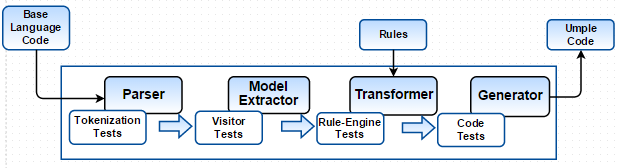
\includegraphics[width=0.9\textwidth]{Figures/testingPhase.png} 
\caption{Umplificator Testing Infrastructure}
\label{fig:testingPhase}
\end{figure}


\subsection{Testing the Base Language Code Parsers}

Testing the Umplificator parser is centered on the creation of the AST DOM from base language code. Our tests ensure that Base Language code is parsed and tokenized as we expect.

A simple parser test is shown below that verifies that the list of detailed problem reports (warnings, or compilation errors) noted by the compiler during the parsing or the type checking of the compilation unit (file) is what we expect.
In this particular example, we are expecting 2 problems (compilation errors) since the input compilation unit contains two errors at two different locations in the code.

\begin{lstlisting}[style=java]
@Test
public void simpleFileWithTwoErrors()
{
  File testFile = new File(pathToInput+"SimpleFileWithTwoErrors.java");
  String code = SampleFileWriter.readContent(testFile);
  JavaParser javaParser = new JavaParser(); // JDT Parser
  CompilationUnit unit  = javaParser.parseUnit(code);
  Assert.assertEquals(2,unit.getProblems().length());
}
\end{lstlisting}

The pattern for parser-related test is as follows:

\begin{lstlisting}[style=java]
@Test
public void parserTestX()
{
  // Step 1: Load external source file (Java or C++ file)
  // Step 2: Parse file (ensure parsing successful) 
  // Step 3: Verify tokenization
  // Step 4: Clean up
}
\end{lstlisting}

\subsection{Testing the Model Extractor}

Testing the model extractor ensures that from the tokens obtained through the parser we obtain a valid base language model representation (e.g. Java model, Umple model, CPP model). In particular, as we have implemented a Visitor (Visitor software design pattern) to traverse the different elements of the retrieved Base Language model, our tests ensure that the visitors return the desired number of elements.

For instance, if the test input file contains: 

\begin{lstlisting}[style=java, label={lst:inputVisitor}, caption=Java input file for test.]
package cruise.umplificator.visitorTestFiles;

 import java.util.*;
 import java.io.*;

 @SuppressWarnings("unused")
 public class InputForVisitorTest { 

  boolean result = true;
  char capitalC = 'C';
  byte b = 100;
  short s = 10000;
  int i = 100000;
  double d1 = 123.4;
  long creditCardNumber = 1234_5678_9012_3456L;

  InputForVisitorTest () { }

  InputForVisitorTest(byte b) {
   this.b=b;
  }

  public int getB(){
   return b;
  }
}
\end{lstlisting}

in the following unit test we assert that the (Java) visitor returns: 7 field declarations (Lines 17-20), 2 import declarations(Lines 23-27), 3 method declarations (Lines 37-41) and a package name 'cruise.umplificator.visitorTestFiles' (Line 30-34).

\begin{lstlisting}[style=java]
public class JavaVisitorTest {

	String pathToInput;
	JavaClassVisitor visitor ;
	
	@Before
	public void setUp() throws Exception {
		pathToInput = SampleFileWriter.rationalize("test/cruise/umplificator/visitorTestFiles/");
		File testFile = new File(pathToInput+"InputForVisitorTest.java");
		String code = SampleFileWriter.readContent(testFile);
		JavaParser javaParser = new JavaParser();
		CompilationUnit unit  = javaParser.parseUnit(code);
		visitor = javaParser.getJavaVisitor();
	}
	
	@Test
	public void field_declarations_returned_in_java_file()
	{
		Assert.assertEquals(7, visitor.numberOfFieldDeclarations());
	}
		
	@Test
	public void imports_returned()
	{
		int nbImports = visitor.numberOfImportDeclarations();
		Assert.assertEquals(2, nbImports);
	}
	
	@Test
	public void packages_returned()
	{
	    String packageName = visitor.getPackageDeclaration().getName().getFullyQualifiedName();
		Assert.assertEquals("cruise.umplificator.visitorTestFiles", packageName);
	}

	@Test
	public void methods_returned()
	{
		int nbMethods = visitor.numberOfMethodDeclarations();
		Assert.assertEquals(3, nbMethods);
	}
	
\end{lstlisting}

\subsection{Testing the Transformer}

Testing the \textbf{transformer} involves ensuring that our Rule-Engine receives the input, fires the corresponding mapping rules and produces the expected output.
For instance, if the input of our tests below is the Java class in Listing \ref{lst:inputVisitor}, we expect all our assertions to pass. In particular:

\begin{itemize}
\item Line 12-23: In the \textit{setUp()} method of our test, we parsed the input file and create an Umple class that is inserted into the working memory of the Rule Engine (Line X). Note that in Line Y  the desired \textbf{level of refactoring} includes umple attributes(and excludes Umple associations) since the goal of this test class is to ensure the correct mapping between variables possessing certain characteristics and Umple Attributes.

\item Line 26-28: The unit test \textit{testNumberOfObjectsInWorkingMemory} ensures that at this point of time, there is only one element in the working memory (the umple class inserted in Line 22).

\item Line 21-63: The unit test \textit{testCorrectMappingBetweenPrimitiveField2UmpleAttribute} validates the mappings between the Java fields (input) and the Umple attributes. 

\item In Lines 33-35 the fields declarations of the Java class are inserted into the Working Memory. 

\item Line 37: The DROOLS rules are fired. 

\item Line 47-62: We assert that the Rule Engine has correctly created the umple attributes. We ensure that the name and type of field has been correctly assigned to the Umple attribute.

\item Line 65-74: The unit test \textit{testCorrectMappingBetweenImport2Depend} also ensures the correct mapping between the input Java import declarations and the Umple depends.

\item In Line 78 we clean the working memory of the Rule Engine.
\end{itemize}


\begin{lstlisting}[style=java]
public class RulesAttributesTypesTest {

	String pathToInput;
	JavaClassVisitor visitor ;
	RuleRunner runner  = new RuleRunner();
	RuleService ruleService= new RuleService(runner);
	KieSession kieSession;
	UmpleClass uClass;
	CompilationUnit compilationUnit;
	
	@Before
	public void setUp() throws Exception {
		pathToInput = SampleFileWriter.rationalize("test/cruise/umplificator/visitorTestFiles/InputForVisitorTest.java");
		File testFile = new File(pathToInput);
		String code = SampleFileWriter.readContent(testFile);
	   	visitor = new JavaClassVisitor();
		JavaParser javaParser = new JavaParser();
		javaParser.parseUnit(code);
		visitor = javaParser.getJavaVisitor();
		uClass = new UmpleClass("Test");
	    kieSession = ruleService.startRuleEngine(RefactoringLevel.ATTRIBUTES);
		kieSession.insert(uClass);
	}

	@Test
	public void testNumberOfObjectsInWorkingMemory() {
		Assert.assertEquals(1, kieSession.getObjects().size());
	}
	
	@Test
	public void testCorrectMappingBetweenPrimitiveField2UmpleAttribute() {
		// Insert facts into knowledge base
		for(FieldDeclaration field: visitor.getFieldDeclarations()){
			kieSession.insert(field);
		}
		// Fire rules
		kieSession.fireAllRules();
		// Is not Null
		Assert.assertNotNull( uClass.getAttribute(0));
		Assert.assertNotNull( uClass.getAttribute(1));
		Assert.assertNotNull( uClass.getAttribute(2));
		Assert.assertNotNull( uClass.getAttribute(3));
		Assert.assertNotNull( uClass.getAttribute(4));
		Assert.assertNotNull( uClass.getAttribute(5));
		Assert.assertNotNull( uClass.getAttribute(6));

		// Type has been set correctly
		Assert.assertEquals("Boolean", uClass.getAttribute(0).getType());
		Assert.assertEquals("String", uClass.getAttribute(1).getType());
		Assert.assertEquals("Integer", uClass.getAttribute(2).getType());
		Assert.assertEquals("Integer", uClass.getAttribute(3).getType());
		Assert.assertEquals("Integer", uClass.getAttribute(4).getType());
		Assert.assertEquals("Double", uClass.getAttribute(5).getType());
		Assert.assertEquals("Double", uClass.getAttribute(6).getType());
		// Name has been correctly set
		Assert.assertEquals("result", uClass.getAttribute(0).getName());
		Assert.assertEquals("capitalC", uClass.getAttribute(1).getName());
		Assert.assertEquals("b", uClass.getAttribute(2).getName());
		Assert.assertEquals("s", uClass.getAttribute(3).getName());
		Assert.assertEquals("i", uClass.getAttribute(4).getName());
		Assert.assertEquals("d1", uClass.getAttribute(5).getName());
		Assert.assertEquals("creditCardNumber", uClass.getAttribute(6).getName());
	}
	
	@Test
	public void testCorrectMappingBetweenImport2Depend() {
		for(ImportDeclaration importDecl: visitor.getImportDeclarations()){
			kieSession.insert(importDecl);
		}
		kieSession.fireAllRules();
		Assert.assertEquals(2, uClass.getDepends().size());
		Assert.assertEquals("java.util.*", uClass.getDepends().get(0).getName());
		Assert.assertEquals("java.io.*", uClass.getDepends().get(1).getName());
	}
	
	@After
	public void tearDown() throws Exception {
		runner.dispose();		
	}
}
\end{lstlisting}

\subsection{Testing the Umple Code Generator}

Testing the code generator involves asserting that from a input file we obtain the expected umple file. Briefly, we
compare the content of an umple file as generated by the Umplificator and the expected umple file. 

\begin{lstlisting}[style=java]
	@Test
	public void JavaToUmple_VariablesToAttributes_003(){
		String fileName = "003_JavaToUmple_VariablesToAttributes";
		File javaFile = new File(pathToRoot+fileName+"_java.java"); //INPUT
		File umpleFile = new File(pathToRoot+fileName+"_umple.ump"); //OUTPUT
		// Umplify file. Process must succeed!
		assertTrue(umplificator.umplifyElement(javaFile));
		// Get the output content
		assertOuputAndFile(umpleFile);
		// Clean files 
		filesToDelete.add(fileName);
	}
	
	// Helper Functions
	public void assertOuputAndFile(File expectedContentFile)
	{
		try {
			String inputFileContent = FileUtils.readFileToString(expectedContentFile);
			String outputModel  = umplificator.getOutputModel().getCode();
			assertEquals(inputFileContent, outputModel);
		} catch (IOException e) {
			fail();
		}
	}
\end{lstlisting}

The test above, performs the umplification process on the Java input file, and compares the content of the code produced by the Umplificator with the code of the expected umple file. The comparison is done with the help of method \textit{assertOuputAndFile}.

Testing the different components of our infrastructure allows for better defect management by representing bugs as failing tests, effectively diminishing the time and effort required to perform regression. Furthermore, this multi-level testing helps to make sure that a change or addition of a new feature doesn't break any existing functionality and if there is any bug to quickly locate the defective component. In fact, when a defect is uncovered, it might be one of the following:

\begin{enumerate}
\item Defect in the way the base language code is tokenized and converted into an abstract syntax tree.
\item Incorrect population of the base language metamodel instance from the tokenized language.
\item Inappropriate behavior of the Rule-Engine.
\item Syntax errors in the generated Umple code.
\item Semantic errors in the generated base language code (from the umplified model).
\end{enumerate}

\section{Pre-Validation Phase}

As is customary when introducing a new tool in software engineering, we have tested our umplificator using our own repository of examples. These collection of \textbf{umple} examples, currently 42 ranging from Banking systems to Warehouse control systems is available from review online at \cite{umpleexamples} and was used to generate the Java 'toy examples'. The process is illustrated in Figure \ref{fig:preValidation}. The goal of this pre-validation phase is to assert that the \textbf{UmpleModel} is semantically identical to the \textbf{UmpleModel'} which is the generated output of the Umplificator.
 
\begin{figure}[h]
\centering
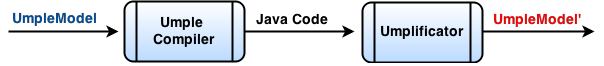
\includegraphics[width=0.75\textwidth]{Figures/preValidation.png} 
\caption{The Pre-Validation Phase: Comparing UmpleModel and UmpleModel'}
\label{fig:preValidation}
\end{figure}

Table \ref{table:umpleexamples} presents the umple examples used in our first phase of validation as well as  some statistics about them (number of lines of code of the Umple model, the number of lines of code of the corresponding Java system and the number of Java classes).

\begin{table}[h]
\caption{Toy examples used for first phase of validation}
\label{table:umpleexamples}
\begin{tabularx}{\textwidth}{l|YYY}
\toprule
\rowcolor[HTML]{BBDAFF}
\textbf{Name} & \textbf{\#LOC of Umple Model} & \textbf{\#LOC of Java system} & \textbf{\# of Java Files} \\ \hline
2DShapes & 44 & 509 & 9\\ \hline
AccessControl & 67 & 1560 & 6\\ \hline
Accidents & 42 & 730 & 4\\ \hline
Accommodations & 102 & 2215 & 9\\ \hline
AfghanRainDesign & 132 & 2610 & 13\\ \hline
Airline & 51 & 1800 & 8\\ \hline
Banking System A & 87 & 2400 & 13\\ \hline
Banking System B & 74 & 1650 & 12\\ \hline
Canal System & 69 & 2222 & 14\\ \hline
Decisions & 148 & 4153 & 15\\ \hline
Card Games (Oh Hell and Whist) & 134 & 2051 & 8\\ \hline
Claim (Insurance) & 19 & 408 & 2\\ \hline
Community Association & 68 & 1591 & 9\\ \hline
Co-op Education System & 69 & 2420 & 10\\ \hline
DMM Overview & 59 & 1165 & 10\\ \hline
DMM Source Object Hierarchy & 91 & 1774 & 16\\ \hline
DMM Relationship Hierarchy & 135 & 1119 & 31\\ \hline
DMM CTF & 93 & 932 & 4\\ \hline
Election System & 83 & 2875 & 11\\ \hline
Elevator System A & 42 & 1307 & 4\\ \hline
Elevator System B & 56 & 1971 &11\\ \hline
Genealogy A & 29 & 670 & 2\\ \hline
Genealogy B & 32 & 945 & 2\\ \hline
Genealogy C & 36 & 1017 & 3\\ \hline
Geographical Information System & 52 & 1174 & 11\\ \hline
Hospital & 65 & 1923 & 9\\ \hline
Hotel & 47 & 1888 & 10\\ \hline
Insurance & 63 & 1417 & 10\\ \hline
Inventory Management & 44 & 1753 & 7\\ \hline
Library & 42 & 1595 & 10\\ \hline
Mail Order System- Client Order & 38 & 1895 & 8\\ \hline
Manufacturing Plant Controller & 84 & 3089 & 11\\ \hline
Pizza System & 67 & 1555 & 9 \\ \hline
Police System & 64 & 3186 & 10\\ \hline
Political Entities & 32 & 842 & 5\\ \hline
Real Estate & 79 & 2071 & 8\\ \hline
Routes and Locations & 127 & 2089 & 9\\ \hline
School & 18 & 397 & 9\\ \hline
TelephoneSystem & 38 & 1838 & 7\\ \hline
University System & 32 & 1206 & 4\\ \hline
Vending Machine & 97 & 1696 & 8\\ \hline
WarehouseSystem & 83 & 2831 & 12\\ \hline

\hline
\end{tabularx}
\end{table}

For instance, the \textit{'Access Control Example'} representing a system for managing access to facilities is comprised of 6 classes, 8 associations, 10 attributes. The umple model is presented below together with corresponding visual representation, a UML class diagram generated using our online tool. The unit test comparing the input Umple Model and the umplified model (output) is shown in Listing \ref{lst:acsExample}.

\begin{lstlisting}[style=umpleIn]
namespace access_control;

class FacilityType
{
  code;
  description { Menu, Record, Screen }
  key {code}
}

//Functional_Area
class FunctionalArea
{
  String code;
  0..1 parent -- * FunctionalArea child;
  description { Hr, Finance }
  key {code}  
}

//Facility_Functional_Area
association
{
  * FunctionalArea -- * Facility;
}

class Facility
{
  Integer id;
  lazy Time t; 
  * -> 0..1 FacilityType;
  Integer access_count;
  name;
  description;
  other_details;
  
  key {id}
}

class Role
{
  code;
  role_description { Dba, ProjectMgr }
  
  key {code}
}

class User
{
  Integer id;
  * -> 0..1 Role;
  first_name;
  last_name;
  password;
  other_details;
  key {id}
}

associationClass RoleFacilityAccessRight
{
  * Facility;
  * Role;
  CRUD_Value { R, RW }
}
\end{lstlisting}

\begin{figure}[h]
\centering
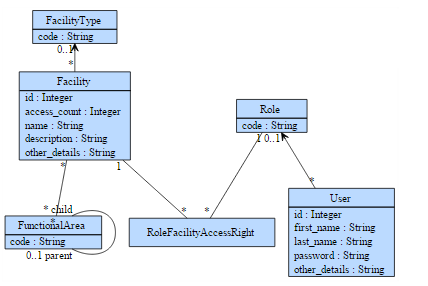
\includegraphics[width=1\textwidth]{Figures/accessControl.png} 
\caption{UML Class diagram of the Access Control system}
\label{fig:preValidation}
\end{figure}

\begin{lstlisting}[style=umpleOut,label={lst:acsExample},caption=Unit test to assert the Access Control Example.]
@Test
public void AccessControlExample(){
	String folderName = "AccessControl";
	File inputFile = new File(pathToRoot+ File.separator +folderName +".ump");
	UmpleFile inputUmpleFile = new UmpleFile(inputFile);
	// Umplify all the files in folder
	List<File> inputFiles = FileHelper.getListOfFilesFromPath(pathToRoot+ File.separator + folderName, new ArrayList<File>());
	// Umplify files. Process must succeed!
	assertTrue(umplificator.umplify(inputFiles));
	// This is the actual model, the one umplified 
	UmpleModel umplifiedModel = umplificator.getOutputModel();
	UmpleModel expectedModel = new UmpleModel(inputUmpleFile);
	expectedModel.run();		
	//1. Class FacilityType
	UmpleClass facilityTypeA = umplifiedModel.getUmpleClass("FacilityType");
	UmpleClass facilityTypeE = expectedModel.getUmpleClass("FacilityType");		
	Assert.assertEquals(1, facilityTypeA.numberOfAttributes());
	Attribute lazyAttributeA = facilityTypeA.getAttribute("code");
	Attribute lazyAttributeE = facilityTypeE.getAttribute("code");	
	assertEquals(lazyAttributeA.getIsLazy(),lazyAttributeE.getIsLazy());
	assertEquals(lazyAttributeA.getType(),lazyAttributeE.getType());		
	// 2. Class User
	UmpleClass userA = umplifiedModel.getUmpleClass("User");
	UmpleClass userE = expectedModel.getUmpleClass("User");	
	Attribute id = userA.getAttribute("id");
	Attribute firstname = userA.getAttribute("first_name");
	Attribute lastname = userA.getAttribute("last_name");
	Attribute other_details = userA.getAttribute("other_details");
	Attribute password = userA.getAttribute("password");
			
	Assert.assertEquals(userA.numberOfAttributes(), userE.numberOfAttributes());
	Assert.assertEquals("Integer", id.getType());
	Assert.assertEquals("String", firstname.getType());
	Assert.assertEquals("String", lastname.getType());
	Assert.assertEquals("String", other_details.getType());
	Assert.assertEquals("String", password.getType());
	// 3. Facility Class
	UmpleClass facilityA = umplifiedModel.getUmpleClass("Facility");
	UmpleClass facilityE = expectedModel.getUmpleClass("Facility");
	Assert.assertEquals(facilityA.numberOfAttributes(), facilityE.numberOfAttributes());
	
	Attribute timeAttr = facilityA.getAttribute("t");
	Attribute idAttr = facilityA.getAttribute("id");
	Attribute accessAttr = facilityA.getAttribute("access_count");
	Attribute nameAttr = facilityA.getAttribute("name");
	Attribute descAttr = facilityA.getAttribute("description");
	Attribute otherAttr = facilityA.getAttribute("other_details");
			
	Assert.assertTrue(timeAttr.isIsLazy());
	Assert.assertFalse(idAttr.isIsLazy());
	Assert.assertFalse(accessAttr.isIsLazy());
	Assert.assertFalse(nameAttr.isIsLazy());
	Assert.assertFalse(descAttr.isIsLazy());
	Assert.assertFalse(otherAttr.isIsLazy());
	// Compare both models, generally
	assertTrue(areModelsEqual(umplifiedModel,expectedModel));
}
\end{lstlisting}

In the test case above, the level of refactoring includes only attributes (Umple associations have not been extracted) so we are interested in the classes, generalizations and the attributes of each class. We assert that the classes have been correctly detected and that the attributes in each class have been correctly extracted (attribute type, attribute name and additional features). For instance, in Line 69 we assert that the attributes is \textbf{lazy}, since the variable is not one of the parameters in the constructor of the Java class \textbf{Facility} (Java code is not shown here).

More on our approach to validation is presented next.

\section{Initial Phase of Validation}

Additionally, as part of our second stage of validation, we tested the Umplificator on various open-source systems written in Java. We use freely available systems to ease comparisons and replications of our evaluation. We provide some information on these systems in Table \ref{umplifiedSystems} including their version, number of lines of code and the number of classes. The last column of the Table indicates whether or not the system has been studied elsewhere. 
Note that the data (statistics on the modeling constructs detected) in those external studies is used to compare the result of our automated tool. Furthermore, we perform '\textbf{manual}' umplification on the systems \emph{that have not been studied before}, the results of the manual umplification are then compared to the results of our '\textbf{automated}' umplification. In fact, the only project that hasn't been studied (reverse-engineered) before is Weka, a very popular suite of machine learning software written in Java. 

\begin{table}[h]
\caption{Open-source systems umplified}
\label{table:umplifiedSystems}
\begin{tabularx}{\textwidth}{l|YYYY}
\toprule
\rowcolor[HTML]{BBDAFF}
\textbf{Name} & \textbf{Version} & \textbf{LOC} & \textbf{\# of Classes}  & \textbf{Reference} \\ \hline
        JHotDraw \cite{jhotdraw}                   & 7.5.1   & 82132   & 694    & Yes       \\ 
 \hline  Weka \cite{wekasvn}                   	   & 3.7.13  & 278642  & 1370   & No        \\ 
\hline   Java Bug Reporting Tool\cite{jbrtsvn} 		& 1.0     & 2629    & 36     & Yes       \\ 
\hline   JEdit\cite{jeditsvn}                   	& 1.12    & 59699   & 234    & Yes       \\ 
\hline   FreeMaker\cite{freemakersvn}               & 2.3.15  & 39864   & 281    & Yes       \\ 
\hline   Java Financial Library\cite{jflsvn}  		& 1.6.1   & 1248    & 27     & Yes       \\ 
\hline   args4j\cite{args4jsvn}                 	 & 2.0.30  & 2223    & 61     & No        \\
\hline
\end{tabularx}
\end{table}

More concisely, for each system studied, we have followed these steps:

\begin{enumerate}
\item We apply the different transformations steps on the input object-oriented system.
\item We run the test suite available for the system to ensure that code compiles and is semantically identical to the original input source code.
\item We run a custom-made code analyzer on the umple system generated (umplified) to obtain the statistics of the detected (extracted) umple constructs (attributes, associations). At this stage, we obtain the number of attributes extracted for each class, their type, as well as the number of all different types of associations.	

	\begin{itemize}
		\item We compare our results with data obtained independently (if any). For instance, JHotDraw has been reverse-engineered and analyzed in other studies \cite{Gueheneuc}. 
		
		\item In the case that the system has not yet been studied in other related work, we 				compare our results with data obtained from manual umplification. That is, we umplify the system without the help of the Umplificator tool. The manual 	umplification, a very time consuming task, is usually performed by another software engineer (undergraduate 			students contributing to the project).
	\end{itemize}
	
\item We compute the \textbf{precision} and \textbf{recall} of the results previously obtained. Precision assesses the number of true constructs (attributes, associations) identified, while recall assesses the number of true constructs missed by our detection algorithms. 

\item We refine our mapping rules to improve the precision of our algorithms. This step mainly concern  tuning the Umplificator. In general, tuning the Umplificator to increase the accuracy includes one or more of the following manual steps:

	\begin{enumerate}
		\item If there is an Umple construct that was missed from the extraction (false negative), we may add a new mapping 			rule to cover this case.
		
		\item If there is an Umple construct that was incorrectly identified (false positive), we may edit the corresponding 			mapping rule.
		
		\item If one of the methods requiring additional transformations (as described in Table 1) was incorrectly refactored.
		
	\end{enumerate}
\end{enumerate}

The following are the definitions we have employed for the precision and recall measures \cite{precisionRecallDef}:

\[  Precision=\frac{(Documented) \cap  (Detected)}{Detected}\]
and \\
\[  Recall=\frac{(Documented) \cap (Detected)}{Documented} \]

 
 In the following sections, we  discuss our experiences with \textbf{JHotDraw} and \textbf{Weka}, the two larger system studied studied.

\section{Second Phase of Validation}

\section{Results}

\subsection{JHotDraw}
 
JHotDraw7 \cite{jhotdraw} is an open source graphic editor that supports operations on many graphics file formats. It makes extensive use of software design patterns and has detailed documentation about its design. We selected JHotDraw for umplification to be able to apply our transformations on documented frameworks and to compare results with the documentation of these frameworks and the analyses performed by other tools [19]. For this research we worked with JHotDraw 7.5.1.
Table X shows the results of detection of at-tributes and associations for the JHotDraw framework. It details the number of classes, the number of attributes and the different types of associations. We also performed a manual analysis to check the accuracy of our algorithms and mapping rules. After improving and refining our rules, we have obtained a precision of 100\%. The refinement consisted of adding the Java idioms that our detection algorithms were not able to catch on the first attempt. For instance, not all the setters in the framework return always a void, some of them return a boolean.

The Umplificator was hence tuned to be able to umplify JHotDraw. With each new system we umplify, we increase the accuracy of the mapping rules as well as the overall effectiveness of the umplificator. In general, tuning the Umplificator to increase the accuracy includes one or more of the following manual steps:

Briefly, the complexity of the tuning depends on the number of false positives and false negatives that the tool generates.

\subsection{Weka}
 
The next system we focused on was the machine learning tool Weka \cite{Weka}. As with our the first attempt at umplifying JHotDraw, our first attempt at automatically umplifying Weka result-ed in a precision of less than 100\% – some idioms it uses were not yet detected by our tool.
For example, some classes in the classifiers package implement add() and remove() methods with different argument types. Also, the Confusion class declares add(RuleSet) and remove(Antecedent) to add and remove a set of rules from the evaluation algorithm. In addition, we detected, after execution of the test suite, that two classes were not compiling due to an unexpected constructor signature.
Initial Umplification results for Weka nonetheless have a precision of 85\% when it comes to attributes and 38\% for 1-to-many associations. Table 8 summarizes the results. Note that a precision of 38\% doesn't mean that the Umplificator has missed 62\% associations of this type. It means that some of them were not correctly transformed into Umple (e.g. incorrect navigability, role names or transformation of accessor/mutator methods). The extensibility and flexibility of our tool allows us to add and refine rules without having to recompile the system.
It is our objective to successively umplify more and more systems, with the hope that eventually our rule base will cover the vast majority of cases needed to successfully umplify new systems the Umplificator is presented with. However, even with a precision in the high 80\% range, our tool serves as a useful tool for umplification. Users can leave some variables un-umplified, or can manually umplify the rest.

